\chapter{Appendix A}\label{appendix_a}

\section{Persona}\label{persona}

\begin{center}
\begin{longtable}{|l|p{10cm}|}
\hline
\textbf{Name} & Alex \\
\hline
\textbf{Age} & 19 \\
\hline
\textbf{Gender} & Male \\
\hline
\textbf{Program} & Computing Science \\
\hline
\textbf{Location} & Singapore Institute of Technology (SIT), Singapore\\
\hline
\textbf{Background} & Alex is the first in his family to step into the realm of higher education. He is enthusiastic about the opportunities that university life offers but is equally apprehensive about the academic hurdles that may come his way. \\
\hline
\textbf{Goals} & Alex aspires to attain a quality education that opens doors to promising career prospects. Additionally, he seeks to establish new connections, make friends, and engage in extracurricular activities for a well-rounded university experience. \\
\hline
\textbf{Pain points} & Alex is concerned about the rigorous academic workload in college, unsure of how to strike a balance between studies and social life. The prospect of making friends and fitting into the university environment adds to his worries. \\
\hline
\textbf{Other important information} & A diligent worker, Alex is determined to succeed in his academic journey. While slightly reserved, he is keen on overcoming shyness to build meaningful connections with his peers. \\
\hline
\end{longtable}
\end{center}


\section{Survey Data}\label{survey_data}

\begin{figure}[H]
  \begin{subfigure}[b]{0.5\textwidth}
    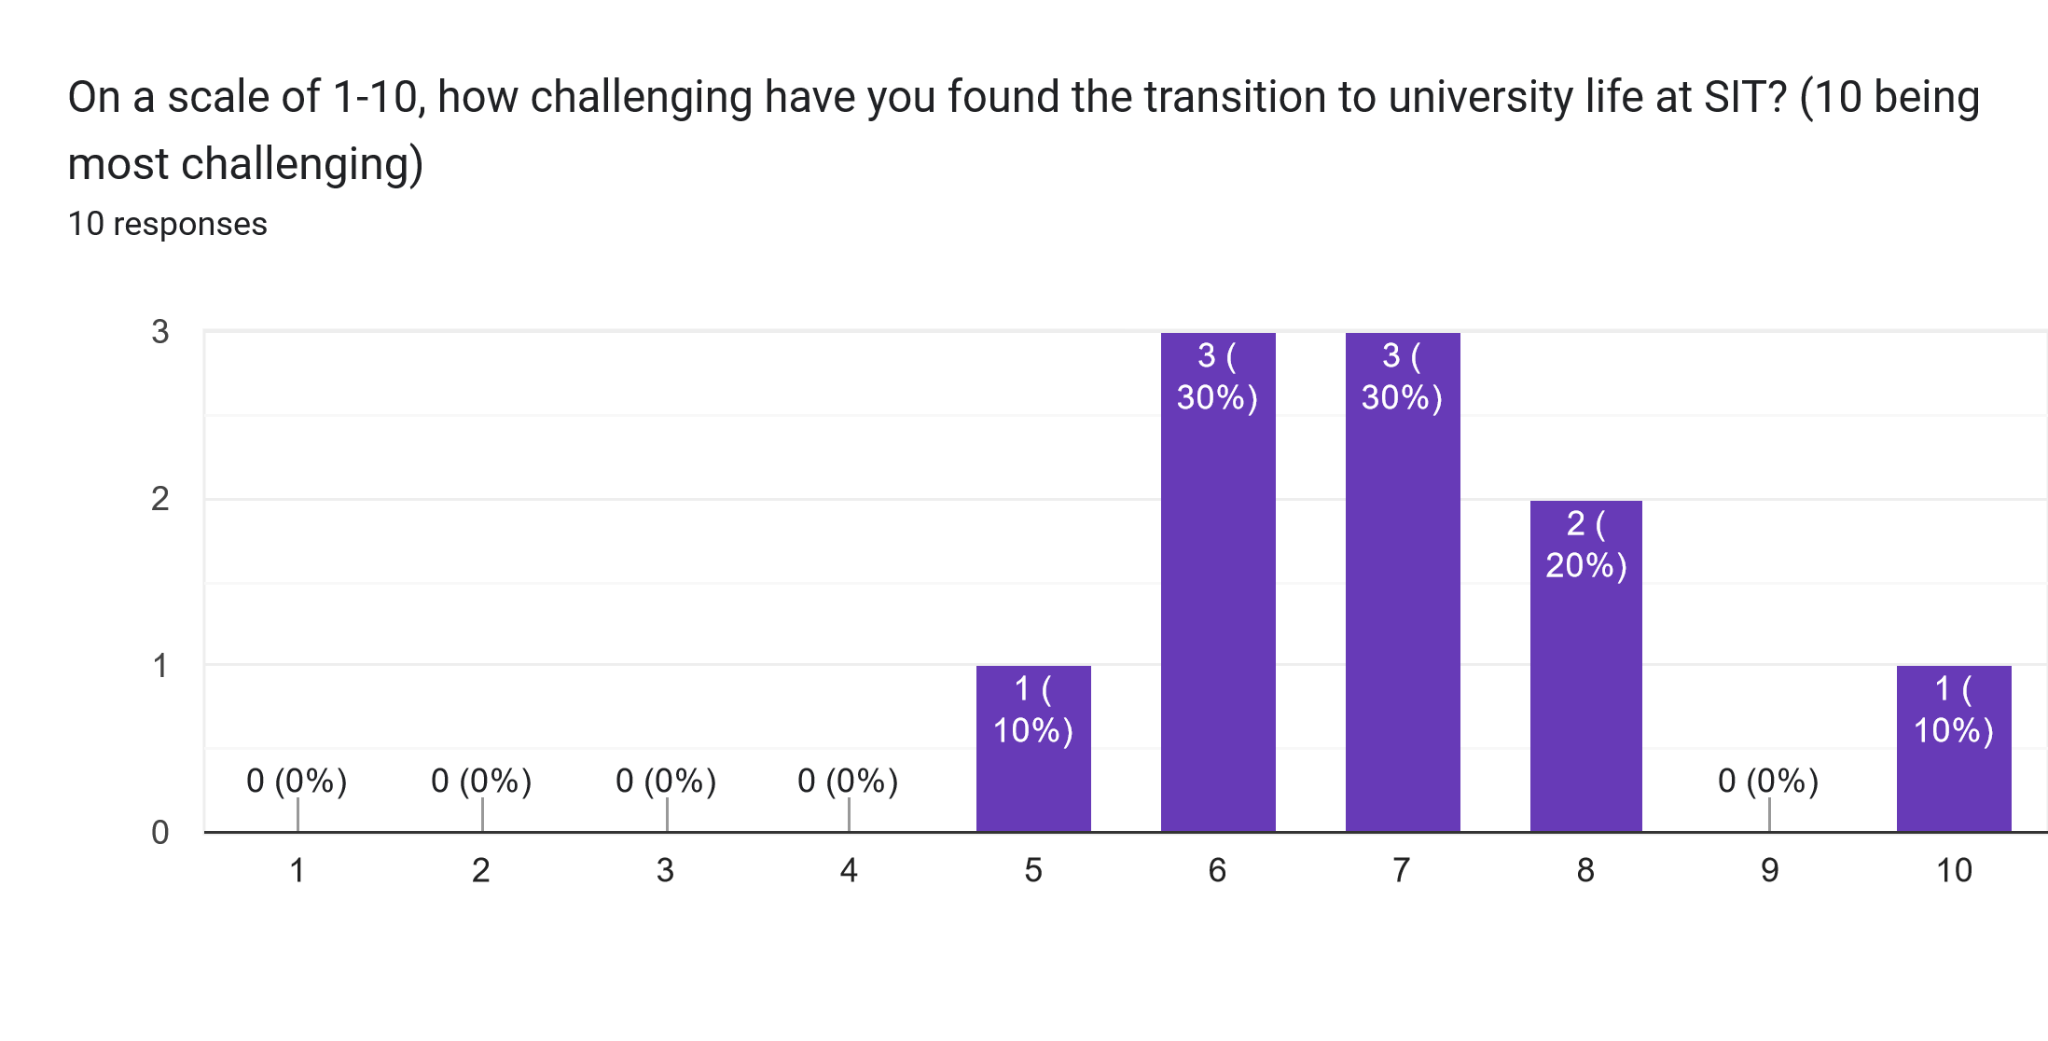
\includegraphics[width=\textwidth]{Figures/Survey/freshie_2.png}
     \caption{\footnotesize Difficulty Level in Transitioning to University for Freshies}
       \label{freshies_difficulty_level_transition}
  \end{subfigure}
  \hfill
  \begin{subfigure}[b]{0.5\textwidth}
    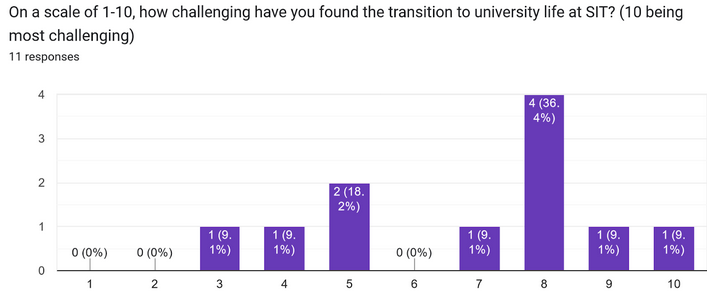
\includegraphics[width=\textwidth]{Figures/Survey/senior_survey.png}
       \caption{\footnotesize Difficulty Level in Transitioning to University for Seniors when they were Freshies}
       \label{senior_difficulty_level_transition}
  \end{subfigure}
  \caption{Difficulty in University Transitioning}
\end{figure}


\begin{figure}[H]
  \begin{subfigure}[b]{0.5\textwidth}
    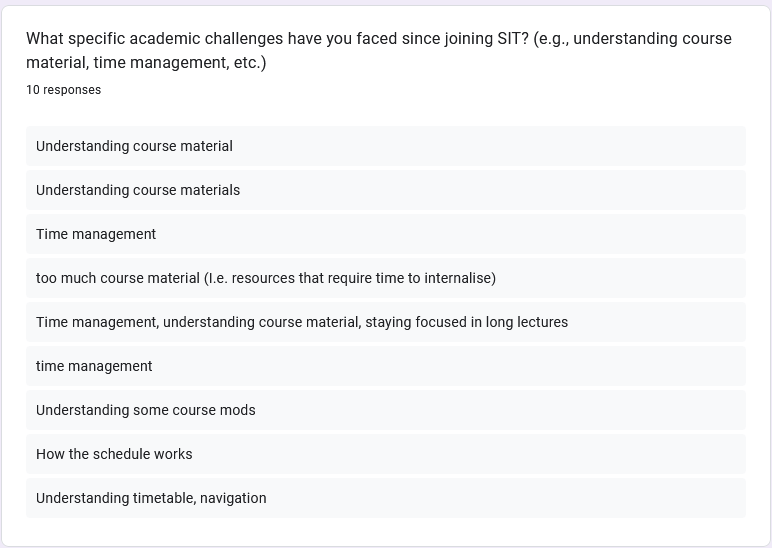
\includegraphics[width=\textwidth]{Figures/Survey/freshie_3.png}
       \caption{\footnotesize Freshie Academic Challenges Faced}
       \label{freshie_acacdemic_difficulty}
  \end{subfigure}
  \hfill
  \begin{subfigure}[b]{0.5\textwidth}
    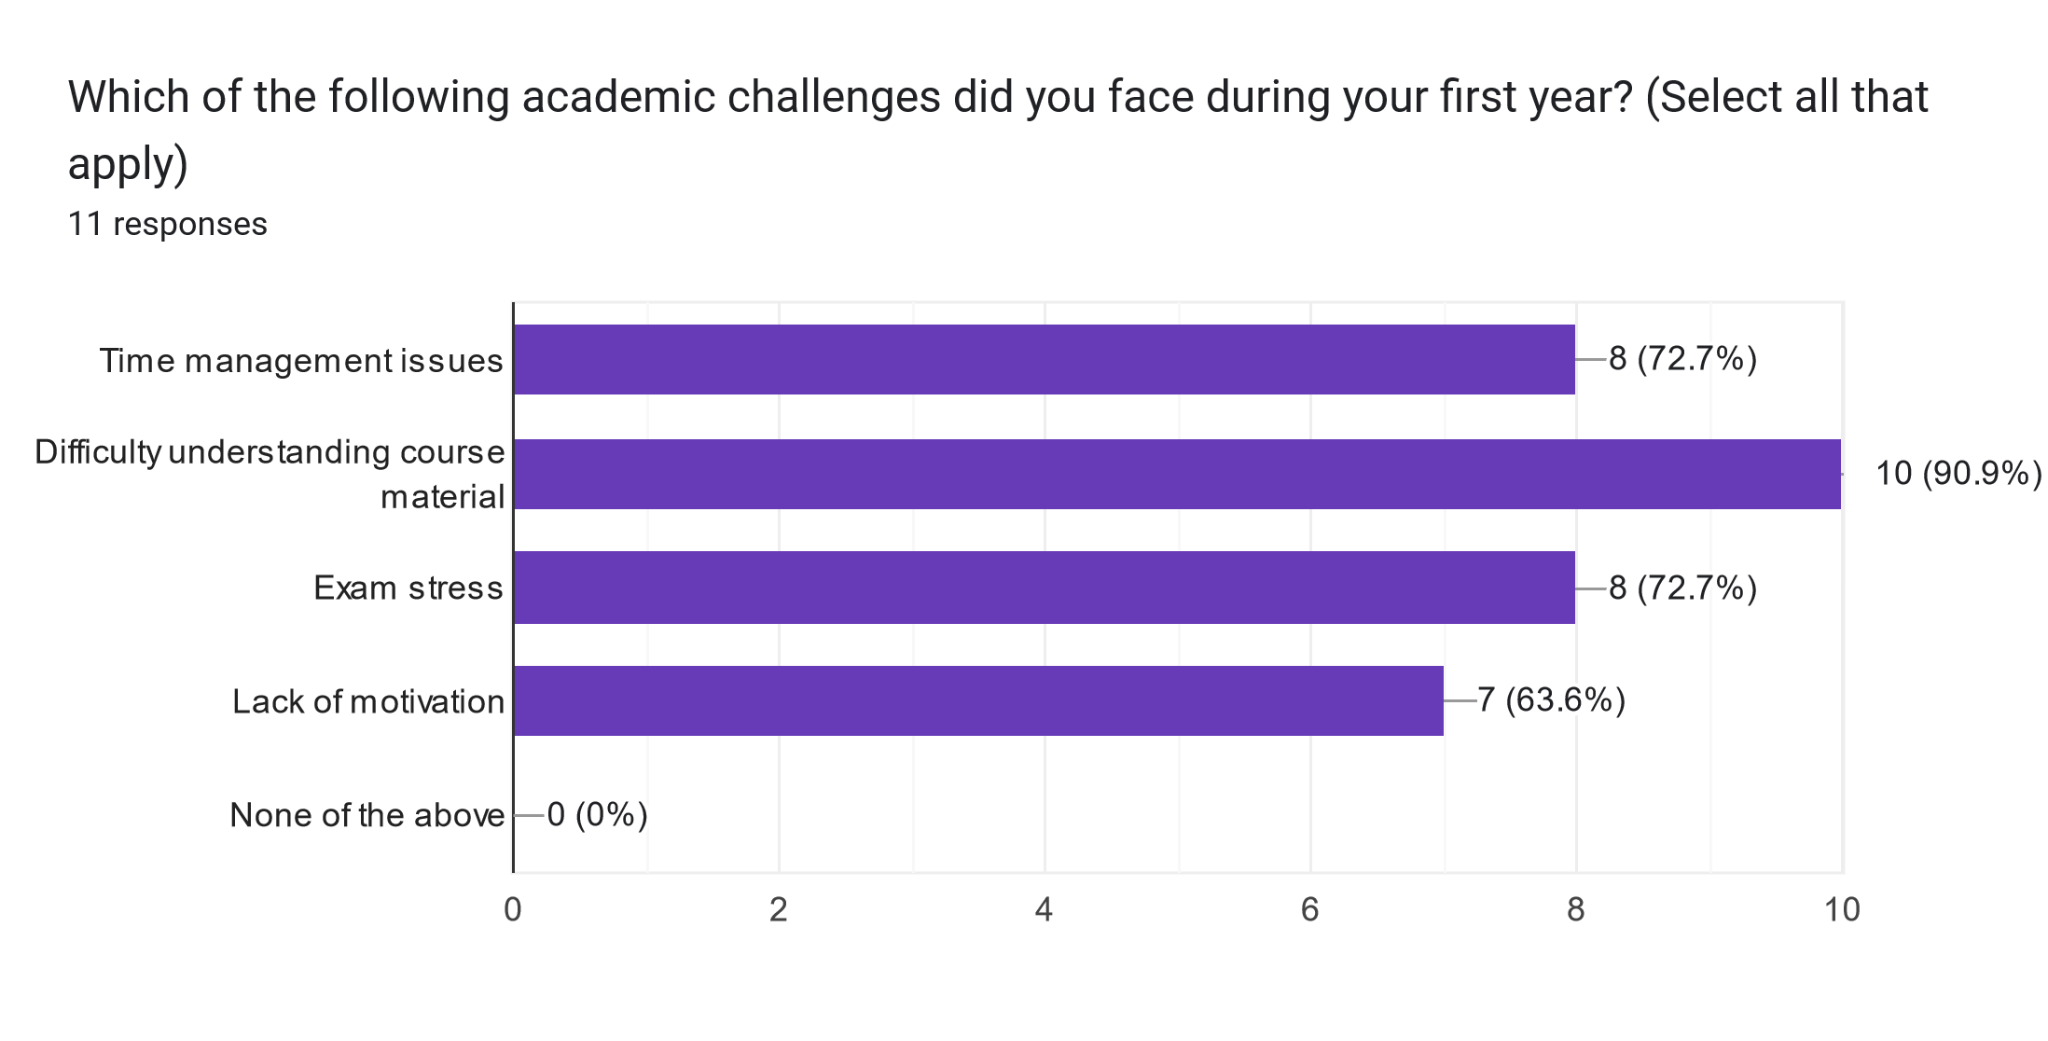
\includegraphics[width=\textwidth]{Figures/Survey/senior_3.png}
       \caption{\footnotesize Senior Academic Challenges Faced when they were Freshies}
       \label{senior_acacdemic_difficulty}
  \end{subfigure}
  \caption{Academic Challenges Faced for Freshies}
\end{figure}


% \begin{figure}[H]
%       \centering
%       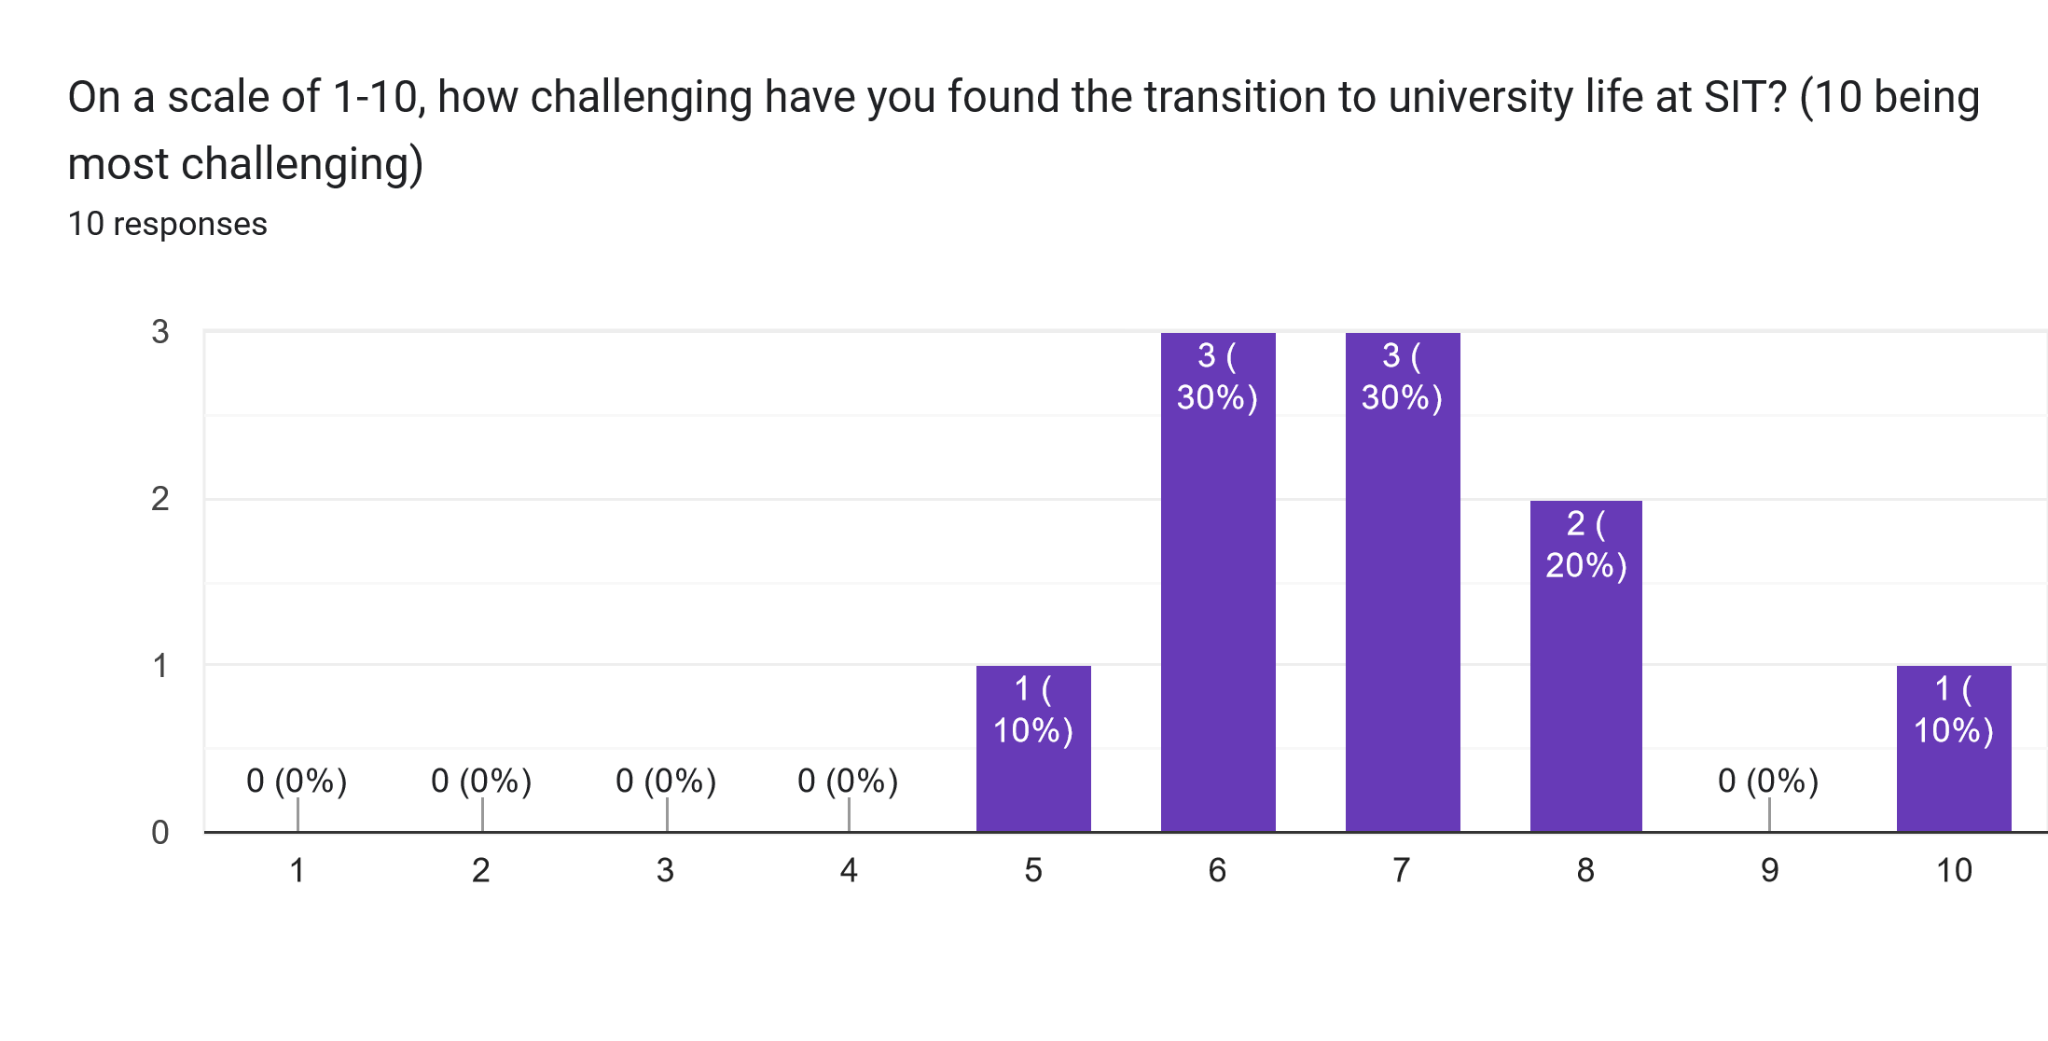
\includegraphics[width=\textwidth]{Figures/Survey/freshie_2.png}
%       \caption{\footnotesize Difficulty Level in Transitioning to University for Freshies}
%       \label{freshies_difficulty_level_transition}
% \end{figure}


% \begin{figure}[H]
%       \centering
%       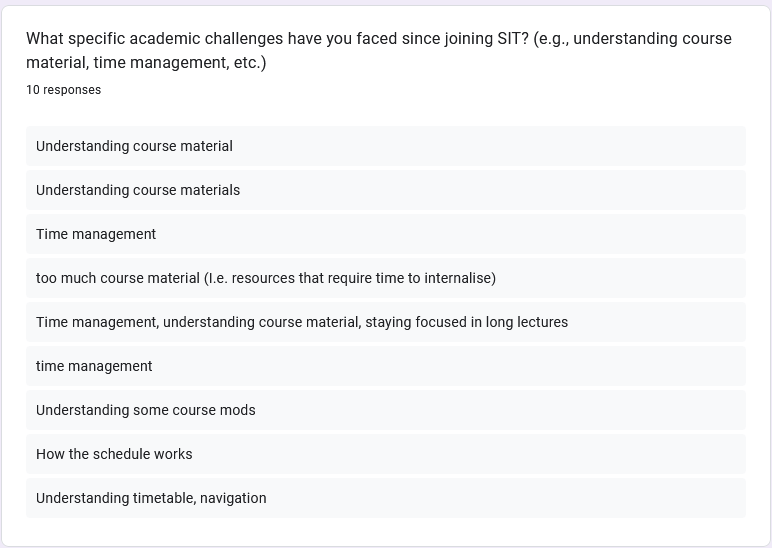
\includegraphics[width=\textwidth]{Figures/Survey/freshie_3.png}
%       \caption{\footnotesize Freshie Academic Challenges Faced}
%       \label{freshie_acacdemic_difficulty}
% \end{figure}


% \begin{figure}[H]
%       \centering
%       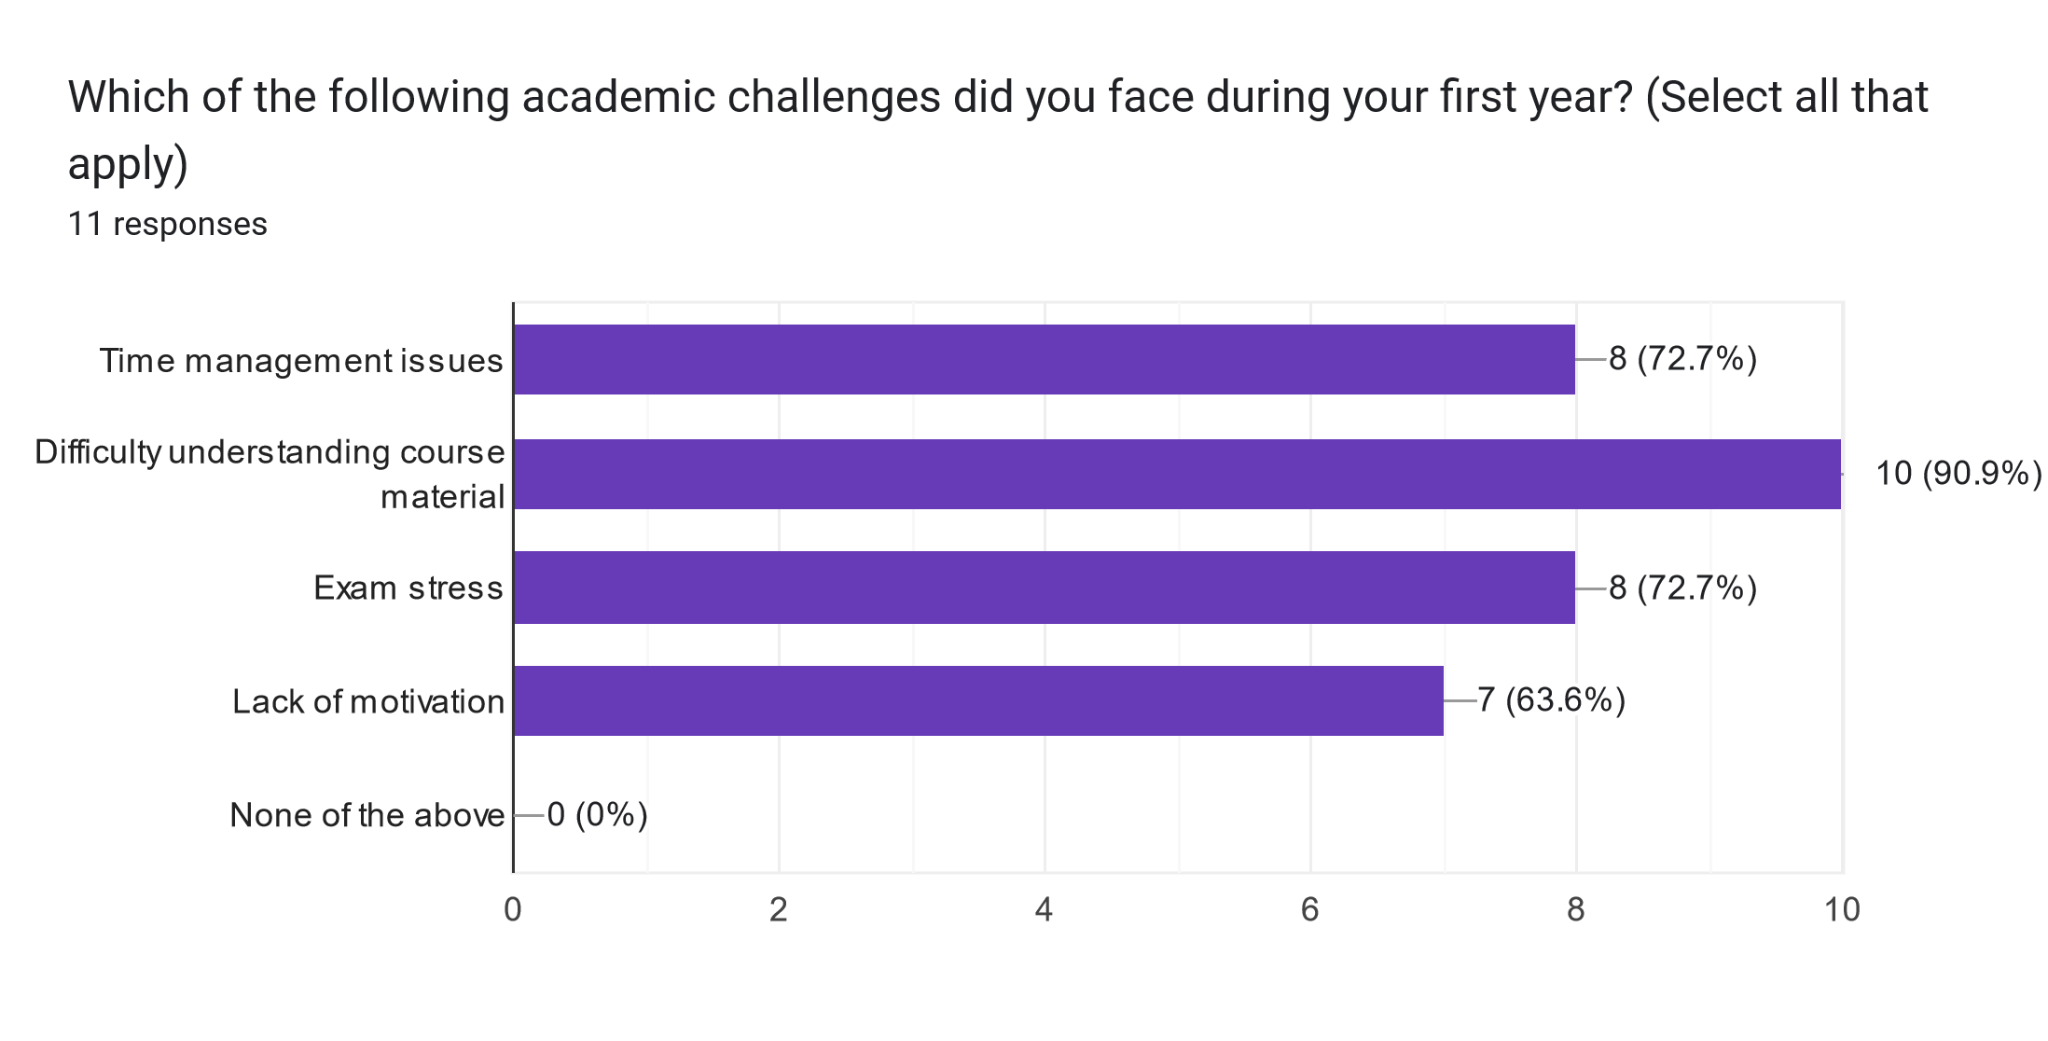
\includegraphics[width=\textwidth]{Figures/Survey/senior_3.png}
%       \caption{\footnotesize Senior Academic Challenges Faced}
%       \label{senior_acacdemic_difficulty}
% \end{figure}


% \begin{figure}[H]
%       \centering
%       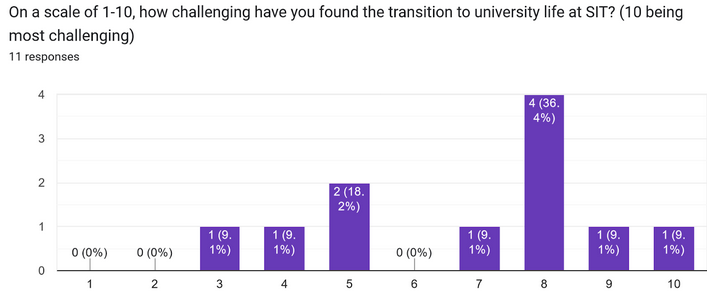
\includegraphics[width=\textwidth]{Figures/Survey/senior_survey.png}
%       \caption{\footnotesize Difficulty Level in Transitioning to University for Seniors when they were Freshies}
%       \label{senior_difficulty_level_transition}
% \end{figure}
